\section{Introduction to the Material}
Upon initial inspection of Maxwell's equations, in particular $\nabla \cdot B = 0$, it appears that the existence of a free magnetic monopole is prohibited due to the fact that all magnetic field lines must form closed loops. In other words a North or South pole cannot exist in the absence of the other, that they must exist as a pair.
\par
\begin{figure}[ht!]
    \begin{center}
        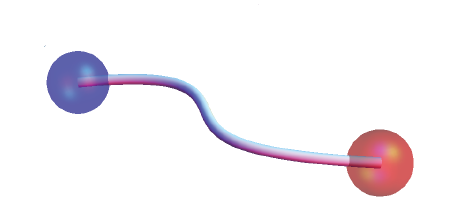
\includegraphics[scale=0.60]{monostring.png}
        \caption[String connecting two monopoles]{String connecting two monopoles}
        \label{fig:gf15}
    \end{center}
\end{figure}
However, we can construct a system where two poles are tethered by an ideally elastic and flexible string-like tube which transports magnetic flux from the south to the north pole. These poles could then be moved arbitrarily far away from each other, and the magnetic field would exclusively emanate from or flow into the ends of the wire. These ends would still interact via Coulomb's law, yet the magnetic field lines still formed closed loops as required by Maxwell's equation $\nabla \cdot B = 0$.
\par
The physicist Paul Dirac published a paper in 1931 predicting the existence of these exact magnetic monopoles.{\cite{b1}}  Dirac showed that if any magnetic monopoles exist, then all electric charge in the universe must be quantized.  The electric charge is in fact quantized, which is consistent with (but does not prove) the existence of magnetic monopoles.
\par
Since Dirac's paper, several monopole searches have been undertaken, most notably the experiments in 1975{\cite{b2}} and 1982.{\cite{b3}}  Both experiments produced events that were initially perceived as being monopoles but these experiments are now regarded as inconclusive.  The question of whether a magnetic monopole exists in free space is still an open one.{\cite{b4}}
\par
The history of physics shows that phenomena in high energy physics have counterparts in condensed matter physics which are described by similar mathematics and during the past few years, physicists have discovered that in synthesized exotic materials known collectively as spin ice, quasi-particles that behave like magnetic monopoles have been observed.
\par
Spin-ice is a geometrically frustrated system of magnetic moments, similar to the frustration of hydrogen ions in water ice.  In the spin-ice structure, these quasi-particles are present in a form of, borrowing the language of monopoles, `monopole/anti monopole' pairs connected by a `Dirac String' of overturned dipoles.
\par
However, in studying these structures experimentally, it is extremely difficult to obtain a spacial image of the spin configurations without altering the state of the system. Instead, in order to observe these quasi-particles what I will be doing is simulating a 2 dimensional frustrated lattice with a kagome structure using Mathematica code provided by the UCD Theoretical Condensed Matter research group.
\clearpage
